\chapter{Methodology}
\section{Introduction}
This chapter contains the methodology of the entire project that has been implemented along with theory regarding why that particular methodology as been used along with images and code snippets.
\section{Dataset}
The dataset used in this project is a premade dataset available on Kaggle. This dataset comprises of a total of 37 hand gestures which include numerical gestures of 0-9, alphabetical gestures for A-Z as well as gestures for a blank space. The Dataset includes both colored images of hand gestures, in the Gesture Image Data, and preprocessed images, in Gesture Image Pre-Processed Data. In this project, only the Gesture Image Data has been used. There are a total of 1500 images for each gesture. The data was distributed for each gesture into three sets, one consisting of 1200 images for training the second consisted of 200 images for validation and 300 images for testing. The size of each image is 50X50 and is located in its specific folder, folders for each gesture are separate.
\begin{figure}[h!]
\centering
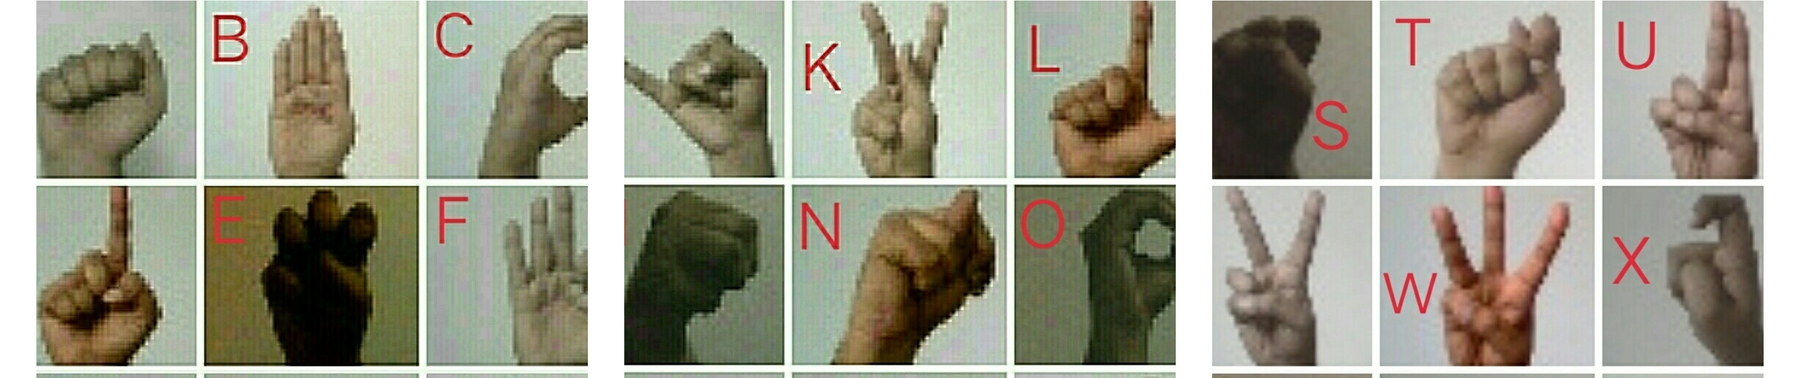
\includegraphics[width=0.5\textwidth]{dataset.jpg}
\caption{\label{fig:frog}Dataset}
\end{figure}

\section{Classifier Used: Convolution Neural Network (CNN)}
CNN (A convolutional neural network) is a deep learning network architecture. It is most commonly used in recognition of data from images and is represented in the form of multidimensional arrays. CNN does not require manual feature extraction and learns directly from the data itself and also assigns weight values to the neurons to be able to differentiation the value of the neurons. The architecture of CNN consists of three layers. The first layer is the convolution layer which passes the input images through a set of convolutional filters for feature extraction. The next layer is the pooling layer where the output of the previous layer is simplified by reducing the dimensions. The last layer is the fully connected layer where the classification of the now simplified data begins, the data is flattened and passed through a network of fully connect neurons that perform mathematical functions on the data. 

\begin{figure} [h!]
\centering
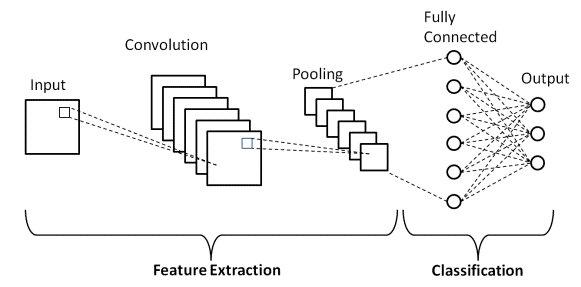
\includegraphics[width=0.7\textwidth]{CNN.png}
\caption{\label{fig:frog}The Layers of a CNN}
\end{figure}

\subsection{Why CNN?}
While there are a number of predecessors and competitors of CNN there are various factors of CNN that make it the better choice for this project.
\begin{enumerate}
\item CNN detect features without human supervision
\item CNN has parameter sharing which reduces the number of computations
\item CNN has dimensionality reducing features
\item CNN is feed forward while RNN is feed backwards
\item It is easy to understand and fast to implement
\item It has the highest accuracy among all the algorithms
\item CNN can handle images while RNN can only handle text
\end{enumerate}

\section{Model of CNN: VGG16}
It is a Convolutional Neural Network (CNN) model. It is built as a deep CNN and is one of the most used image-recognition architectures. //
It involves conversion of RGB to VGR. VGG16 contains total 21 layers with 16 layers having parameters. These 21 layers are divided into 13 Convolution layers, 5 Pooling layers and 3 Dense layers. Convolution layer has a fixed filter of 3x3 with a stride of 1. Max Pooling layer has a fixed filter of 2x2 and contains padding of same and stride of value 2. The first convolution layer has 64 filters, the second has 128 filters, third layer has 256 filters, fourth layer has 512 filters and fifth layer also has 512 filters. MaxPooling is used for the reduction in dimension. 

\section{Keras, TensorFlow, ImageDataGenerator}
Keras is an open-source python interfaced software library which is used to make the implementation of artificial neural networks easier. It is also the interface for the TensorFlow library which is another open-source library. \\
The sequential model for keras has been implemented in this project along with tensorflow. A sequential model is appropriate for a plain stack of layers where each layer has exactly one input tensor and one output tensor\\
Image data generator is used in Preprocessing the images using VGG16 model and then creating batches of them. Vgg16.preprocessinput will convert the input images from RGB to BGR, then will zero-center each color channel with respect to the ImageNet dataset, without scaling.

\begin{figure} [h!]
\centering
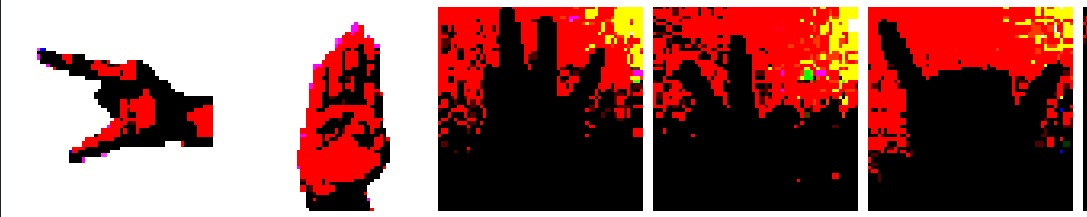
\includegraphics[width=0.7\textwidth]{Plotted data.jpeg}
\caption{\label{fig:frog}Data displayed using plot function}
\end{figure}

\section{Convolution Layer}
The function Conv2D() has been used as a standard convolutional layer that accepts image data. The process of Convolution includes applying a kernel in the input data which is a matrix of size smaller than the matrix size of the input data. This kernel slides along the image based on the input parameters of the function which include the number of output filters, the height and width of the 2D convolution window, the activation function that is applied after performing the convolution, the passing which reduces dimensions and the input shape which specifies the colors and the pixels of the image.

\section{Activation function used: ReLU}
Rectified Linear Unit (ReLU) is a liner function with two types of outputs. If the input is positive, the output of the function is the same as the input. If the input is negative, the output becomes zero.

\begin{figure}[h!]
\centering
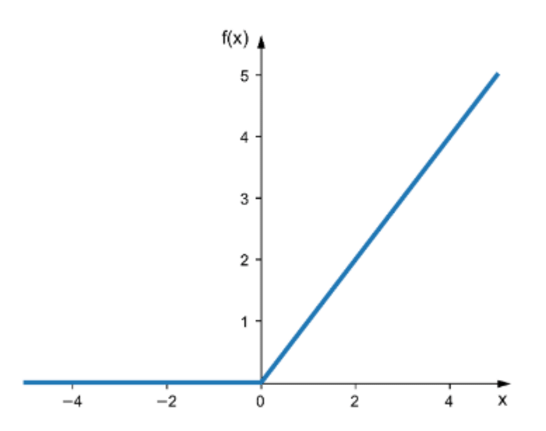
\includegraphics[width=0.5\textwidth]{RELU.png}
\caption{\label{fig:frog}This graphs shows the input (x-axis) and output(y-axis) of ReLU function}
\end{figure}

\section{8.	Pooling Layer}
MaxPool2D() function is used in the pooling layer in this project. This layer reduces the spatial dimensionality of images by reducing the number of pixels in the output from the previous convolutional layer. Pooling layer is always added after a convolutional layer. \\
The function works by taking a block on the input image of the size defined in the parameter as pool size, the max value from this block is taken and stored in the output. The block then moves on based on the stride which is also passed as a parameter. This function is used in the pooling layer as it reduces the computational load and reduces overfitting.

\section{Flatten layer}
Flatten() function is used as it flattens the multi-dimensional input into a single dimension. This is necessary to build a neural network model. The output of this function can then be passed to every single neuron of the model effectively.

\section{Fully Connected layer}
Dense() function is used for changing the dimension of the output by performing matrix vector multiplication. This is where the classification begins. This layer is simply a layer of neurons in which each neuron receives input from all the neurons of previous layer. The neurons in the layer then perform the matrix multiplication and results in an output which is then passed through the activation function. The parameters of the function include the dimensionality of the output and the activation function that is used. Activation function used in this layer is the Softmax() function which is used when we have 2 or more than 2 classes. This function also converts a vector of numbers into a vector of probabilities, the resulting probabilities are used to classify the image as the output contains probabilities of each class.\\
The matrix multiplication operation used is: $output = activation(dot(input, kernel) + bias)$

\section{Compiling}
Model.compile() function is used to configure the model for training. There are three parameters of this function. The first is the optimizer used which is the SGD optimizer. The second parameter is the loss function, categorical Corssentropy is used which assigns one-hot category encoding value in form of 0s and 1 to the data, it also gives a high probability to the correct digit and a low probability to the other digits. The last parameter is the metrics used to evaluate the performance of classification of your model which is accuracy, it is shown as the fraction of predictions our model got right. 

\section{Stopping Training of the model}
ReduceLROnPlateau() function is used to reduce learning rate when a metric has stopped improving. Monitors a quantity and if no improvement is seen for a 'patience' number of epochs, the learning rate is reduced. The Parameters include the quantity to be monitored, the factor by which the learning rate will be reduced and patience which is the number of epochs with no improvement after which learning rate will be reduced.\\
EarlyStopping() function is used to stop training when a monitored metric has stopped improving. Assuming the goal of a training is to minimize the loss. The parameters used include the quantity to be monitored, Minimum change in the monitored quantity to qualify as an improvement, patience which is the number of epochs with no improvement after which training will be stopped, verbosity mode, and mode.\\
Model.fit() function then trains the model for a fixed number of epochs (iterations on a dataset). It takes input data, epochs, call back and validation data as parameters.

\section{Validation and evaluating, saving and predicting of the model}
The same process is repeated for the validation dataset. The data is taken and stored in a variable and the model is evaluated on the validation data to obtain a better result on test data set and printing the accuracy and loss scores\\
The Model is then evaluated using Model.evaluate() function which check whether the model is best fit for the given problem and corresponding data. \\
The model is then saved using Model.save() function which Saves the model in a single HDF5 file. models can be re instantiated in the exact same state, without any of the code used for model definition or training.\\
The model then generates output predictions using Model.predict() function. This method is designed for batch processing of large numbers of inputs. 

\section{Prediction}
Previously saved model is loaded and ROI values assigned. A function is defined by the name of calaccumavg() for the purpose of background subtraction. Background subtraction is a technique for separating foreground elements from the background and is done by generating a foreground mask. This technique is used for detecting dynamically moving objects from static cameras. The running average over the current frame and the previous frames is computed. This gives us the background model and any new object introduced during the sequencing of the video becomes part of the foreground. Cv2.accumulateWeighted() is used to do the calculation. Segmenthand() function is used to segment the hand region from the video sequence. \\
The absolute difference is calculated between the background model and the current frame using the cv2.absdiff() function. The data is then thresholded into a binary image to convert a grayscale image to a binary image, where the pixels are either 0 or 255 (max value) using the cv2.absdiff() function cv2.findContours() is used To find contours. Contours can be explained simply as a curve joining all the continuous points (along the boundary), having same color or intensity. 

\section{Live Data}
Once our CNN is complete, we are testing our CNN on live data by accessing the webcam of the laptop and then recognizing and classifying live data.\\
cv2.VideoCapture() function starts reading a Video from the camera frame by frame. cam.read() is a frame variable which stores frames from camera. Cv2.flip() function frames are flipped to prevent inverted images. ROI is then extracted from the frame and cv2.cvtColor() is used on ROI to convert it to greyscale. Cv2.GaussianBlur() is used to blur the outlines of ROI. \\
If frames are less than 70, the running average is calculated and message is printed to please wait, else hand is segmented. When hand is detected, image is thresholded, contours are drawn, image is resized, colours are converted to greyscale, image is reshaped. The image is now passed for prediction and the prediction is printed
